\documentclass[a4paper, 14pt]{extarticle}%тип документа

%Русский язык
\usepackage[T2A]{fontenc} %кодировка
\usepackage[utf8]{inputenc} %кодировка исходного кода
\usepackage[english,russian]{babel} %локализация и переносы

%отступы 
\usepackage[left=2cm,right=2cm,top=2cm,bottom=3cm,bindingoffset=0cm]{geometry}

%Вставка картинок
\usepackage{graphicx}
\usepackage{wrapfig, caption}
\graphicspath{}
\DeclareGraphicsExtensions{.pdf,.png,.jpg, .jpeg}
\newcommand\ECaption[1]{%
     \captionsetup{font=footnotesize}%
     \caption{#1}}

%Таблицы
\usepackage[table,xcdraw]{xcolor}
\usepackage{booktabs}

%Графики
\usepackage{pgfplots}
\pgfplotsset{compat=1.9}

%Математика
\usepackage{amsmath, amsfonts, amssymb, amsthm, mathtools}

%Заголовок
\author{Подлесный Артём \\ группа 827}
\title{Работа 4.1.1 \\ ИЗУЧЕНИЕ ЦЕНТРИРОВАННЫХ
ОПТИЧЕСКИХ СИСТЕМ}

\begin{document}
\maketitle

\paragraph*{Цель работы:} изучить методы определения фокусных расстояний линз и сложных
оптических систем; определить характеристики оптической системы, составленной из
тонких линз; изучить недостатки реальных линз сферическую и хроматическую аберрации.
\paragraph*{Оборудование:} измерительный оптическая скамья с набором рейтеров, положительные и отрицательные линзы, экран, осветитель с ирисовой диафрагмой, зрительная труба, светофильтры, кольцевые диафрагмы, линейка.

\section{Определение фокусных расстояний тонких линз с помощью
зрительной трубы}

Перед началом работы все оптические системы были отцентрированы. Всего в измерениях участвуют 5 линз, каждая из которых соответсвующе пронумерована. Качественно было определено, что все линзы с 1 по 4 являются собирающими, с увеличивающимся фокусным расстоянием от порядкового номера. 5 линза -- рассеивающая. 

Экспериментальная установка представлена на рис.1. Показанные на схеме величины снимались после получения четкого изображения источника в зрительной трубе.

\begin{figure}[h!]
\begin{center}
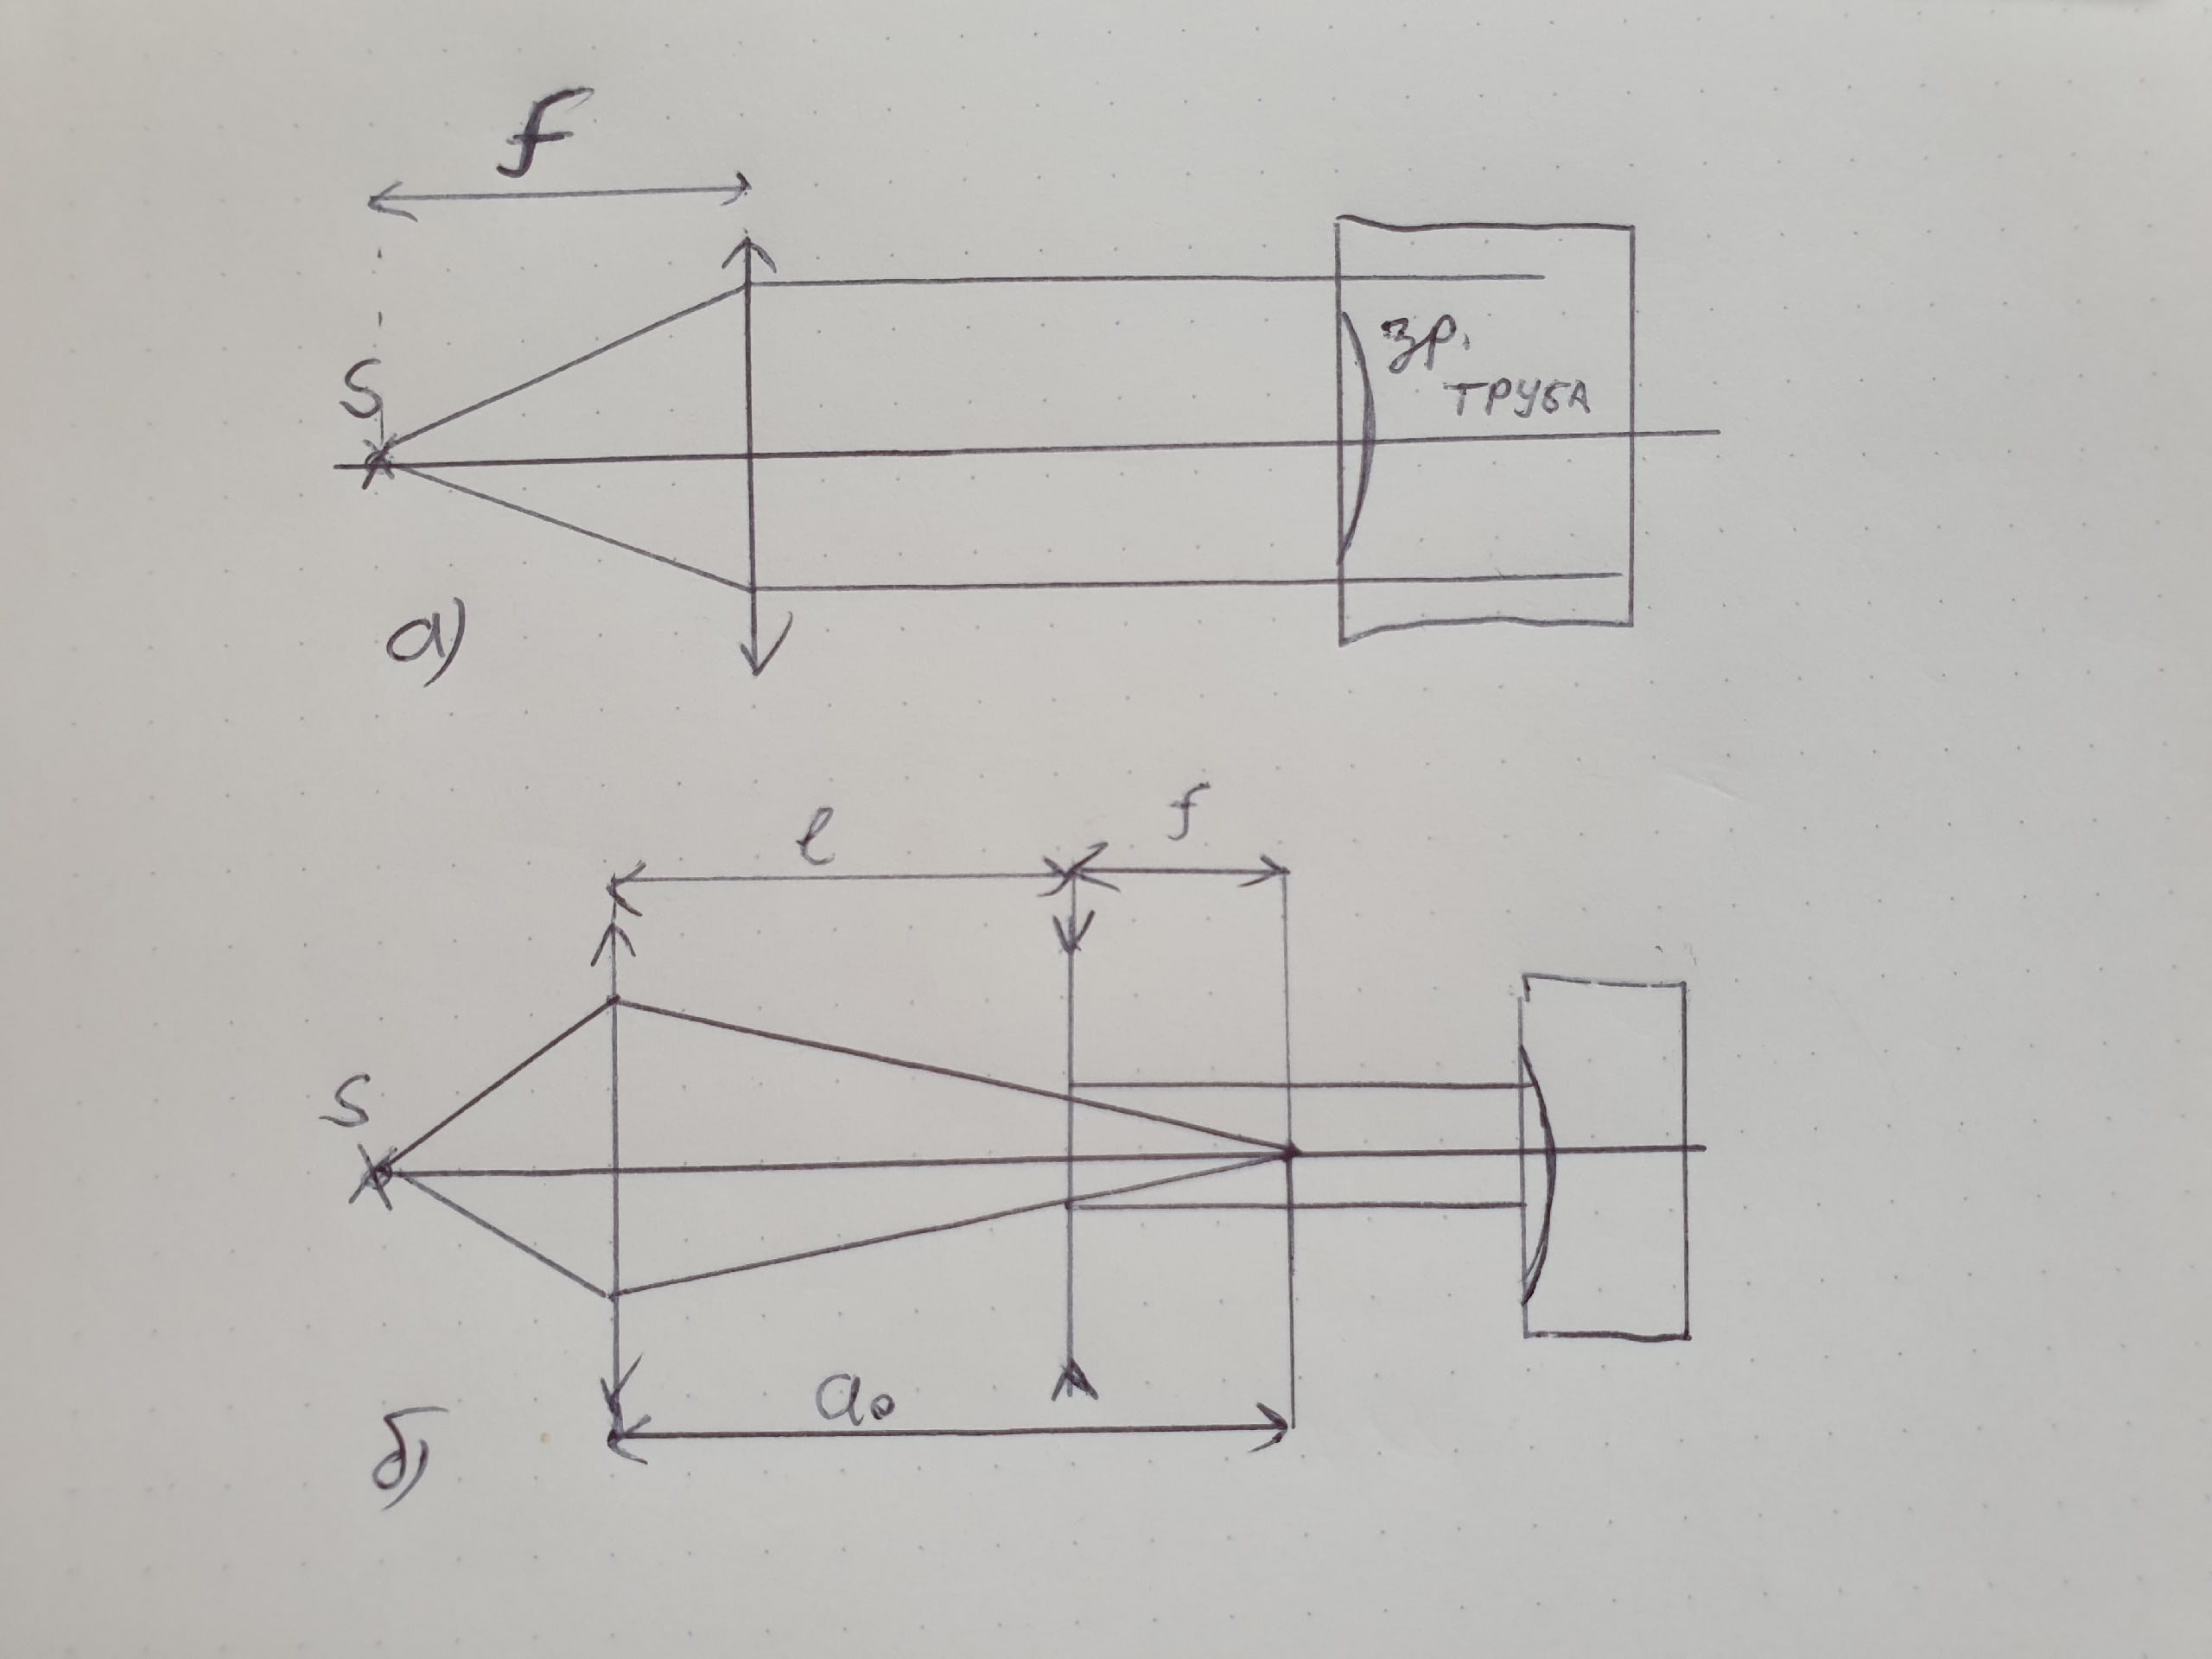
\includegraphics[width=0.8\textwidth]{1}
\end{center}
\ECaption{Экспериментальная установка для определения фокусного расстояния тонкой а)собирающей и б)рассеивающей линз с помощью зрительной трубы. }
\end{figure}

Зрительная труба предварительно установлена на бесконечность (с помощью куртки Булата и коридора). На схеме видно, какие данные снимались для определения фокусного расстояния $f$ линз. Для каждой линзы аналогичные измерения проведены, когда ее повернули другой стороной к источнику (для исключения влияния толщины линз). Данные по измерению каждого фокуса показаны на таблице 1.

\begin{table}[h!]
\begin{center}
\begin{tabular}{|c|c|c|c|c|}
\hline
\rowcolor[HTML]{9698ED} 
Линза & $f_{\text{str}}$, см & $f_{\text{opp}}$, см & $f$, см & $\sigma_f$, см \\ \hline
1     & 7.8           & 7.8           & 7.8     & 0.1            \\ \hline
\rowcolor[HTML]{9698ED} 
2     & 10.8            & 10.5            & 10.7    & 0.2            \\ \hline
3     & 19.6            & 19.1          & 19.4    & 0.2            \\ \hline
\rowcolor[HTML]{9698ED} 
4     & 28.4          & 28.8          & 28.6    & 0.1            \\ \hline
5     & -8.8          & -9.1          & -9.0    & 0.3            \\ \hline
\end{tabular}
\ECaption{$ f_{\text{str}} $ и $ f_{\text{opp}} $ -- фокусы, посчитанные для разных сторон линз. Для рассеивающей линзы были соответственно померяны $l$ и $a_0$, я лишь опустил расчеты.}
\end{center}
\end{table}

\newpage
\section{Определение фокусных расстояний тонких линз при помощи экрана}

\subsection{С помощью метода Бесселя}

Схема метода показана на рис.2. 

\begin{figure}[h!]
\begin{center}
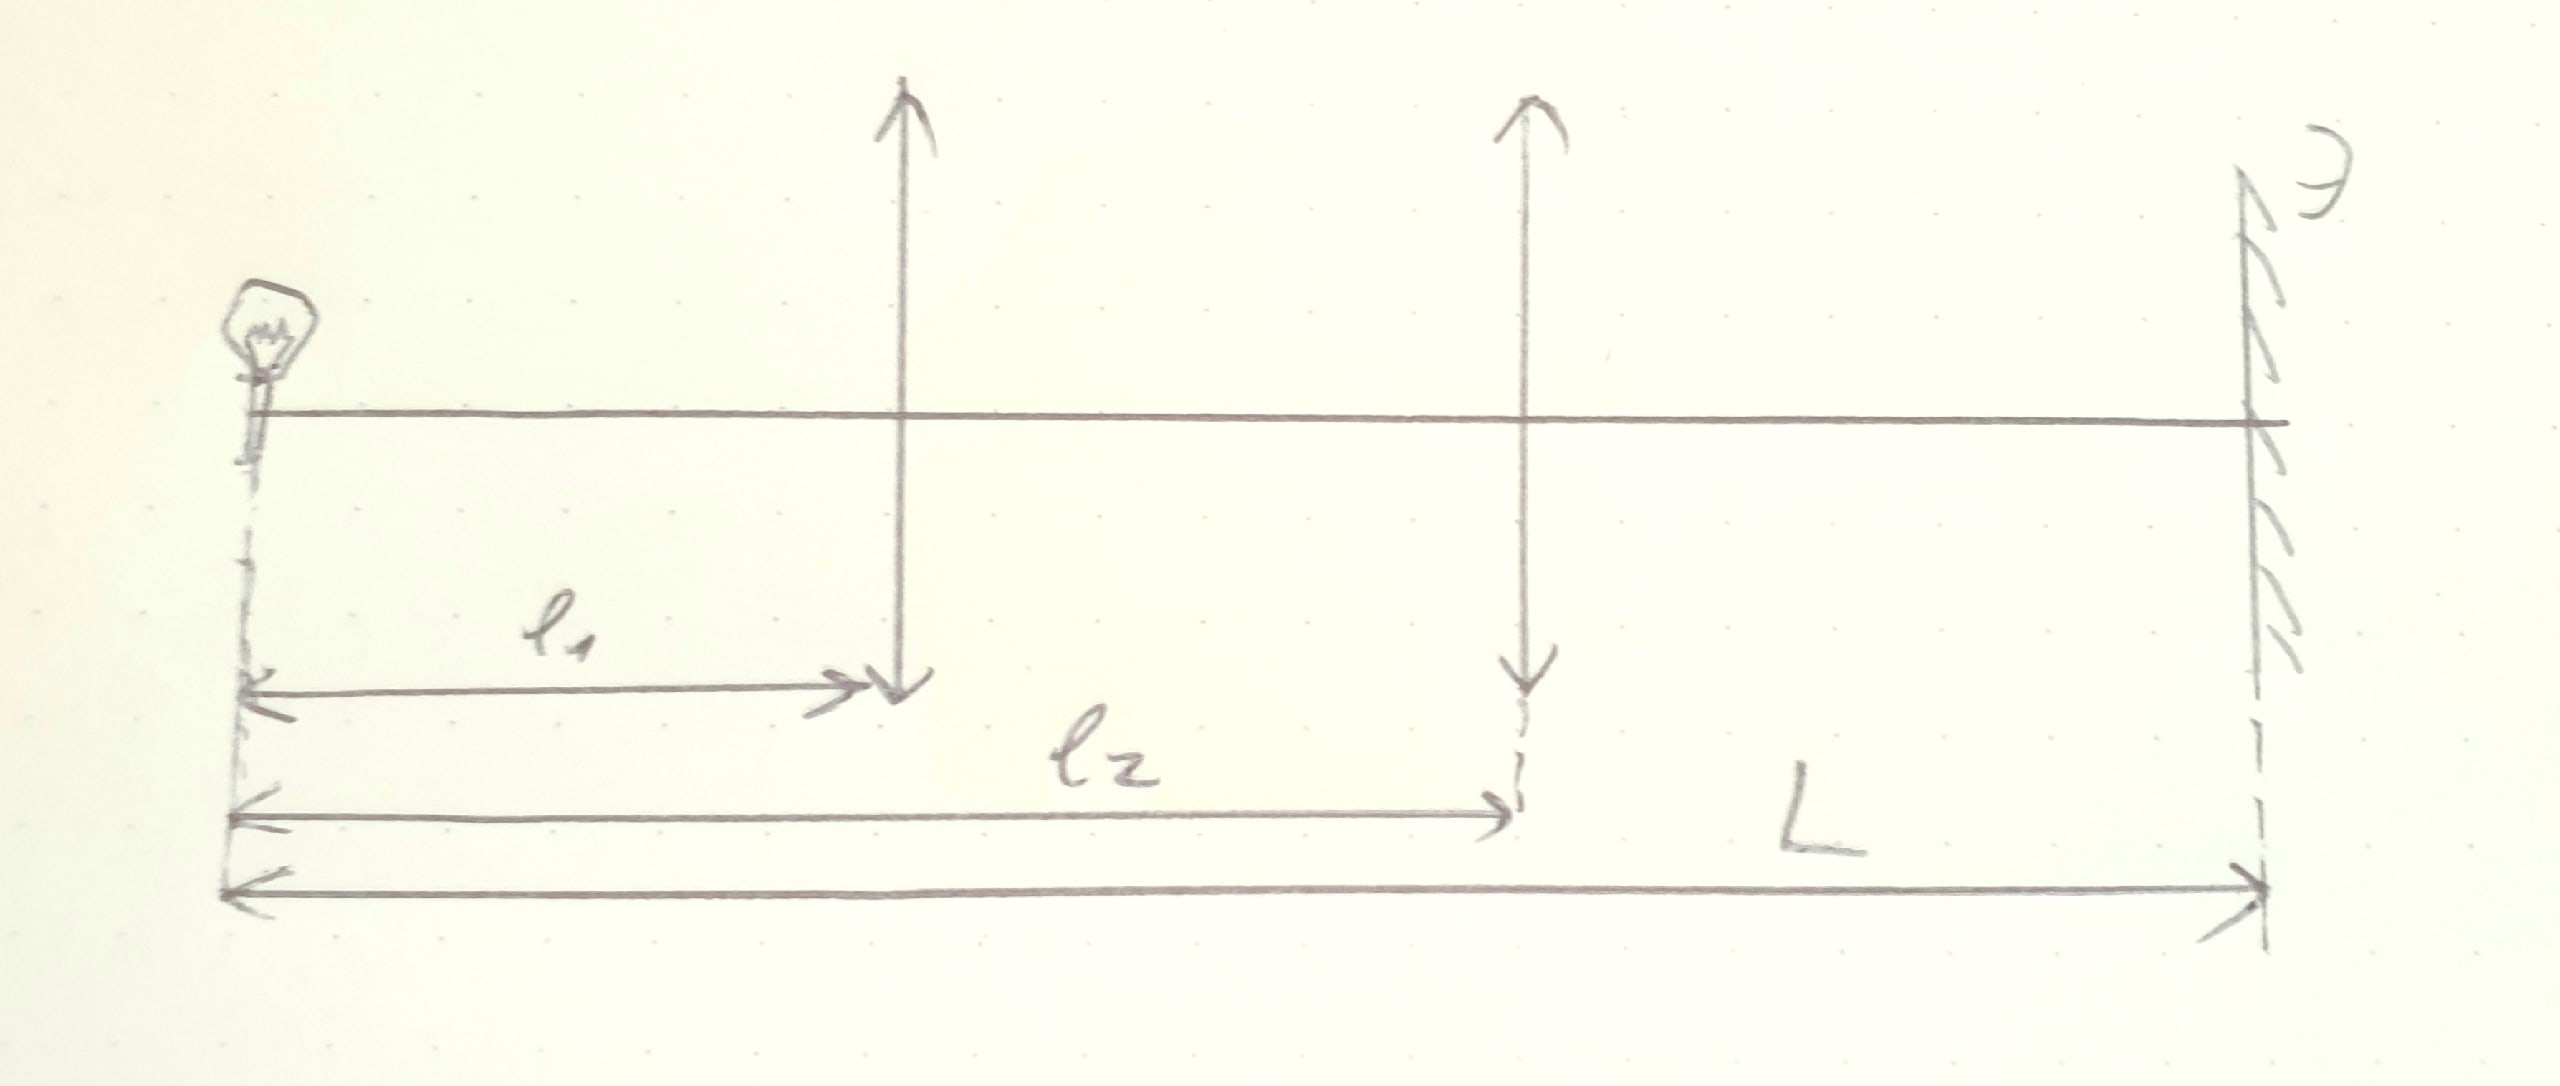
\includegraphics[width=0.9\textwidth]{2}
\end{center}
\ECaption{Схема определения фокусного расстояния собирающей линзы методом Бесселя. В данных обозначениях $l = l_2-l_1$. }
\end{figure}

Суть метода в следующем: пусть $L$ -- расстояние между источником и экраном. Тогда если $l$ -- расстояние между двумя положениями линзы, при котором наблюдается четкое изображения источника на экране, то из формулы тонкой линзы следует, что:
\begin{equation}
f = \dfrac{L^2 - l^2}{4L}.
\end{equation}

Так как таким методом можно определить лишь действительные значения фокусов, то измерялись лишь собирающие линзы. Результаты - на таблице 2.

\begin{table}[h!]
\begin{center}
\begin{tabular}{|c|c|c|c|c|c|}
\hline
\rowcolor[HTML]{9698ED} 
Линза & $L$, см & $l_1$, см & $l_2$, см & $f$, см & $\sigma_f$, см \\ \hline
1     & 43.6    & 9.8       & 33.4      & 7.7     & 0.1            \\ \hline
\rowcolor[HTML]{9698ED} 
2     & 49.8    & 15.1      & 34.3      & 10.6    & 0.1            \\ \hline
3     & 84.1    & 29.3      & 55.3      & 19.0    & 0.1            \\ \hline
\rowcolor[HTML]{9698ED} 
4     & 120.8   & 44.6      & 76.4      & 28.1    & 0.1            \\ \hline
\end{tabular}
\ECaption{Фокусные расстояния линз, измеренные методом Бесселя. Погрешность измерений определяется погрешностью измерений линейки, но в реальности она, конечно, выше.}
\end{center}
\end{table}

\subsection{По формуле тонкой линзы}

В данном эксперименте использовались линзы под номерами 1 и 5 -- с положительным и отрицательным фокусом соответственно. Схема эксперимента представлена на рис.3.

\begin{figure}[h!]
\begin{center}
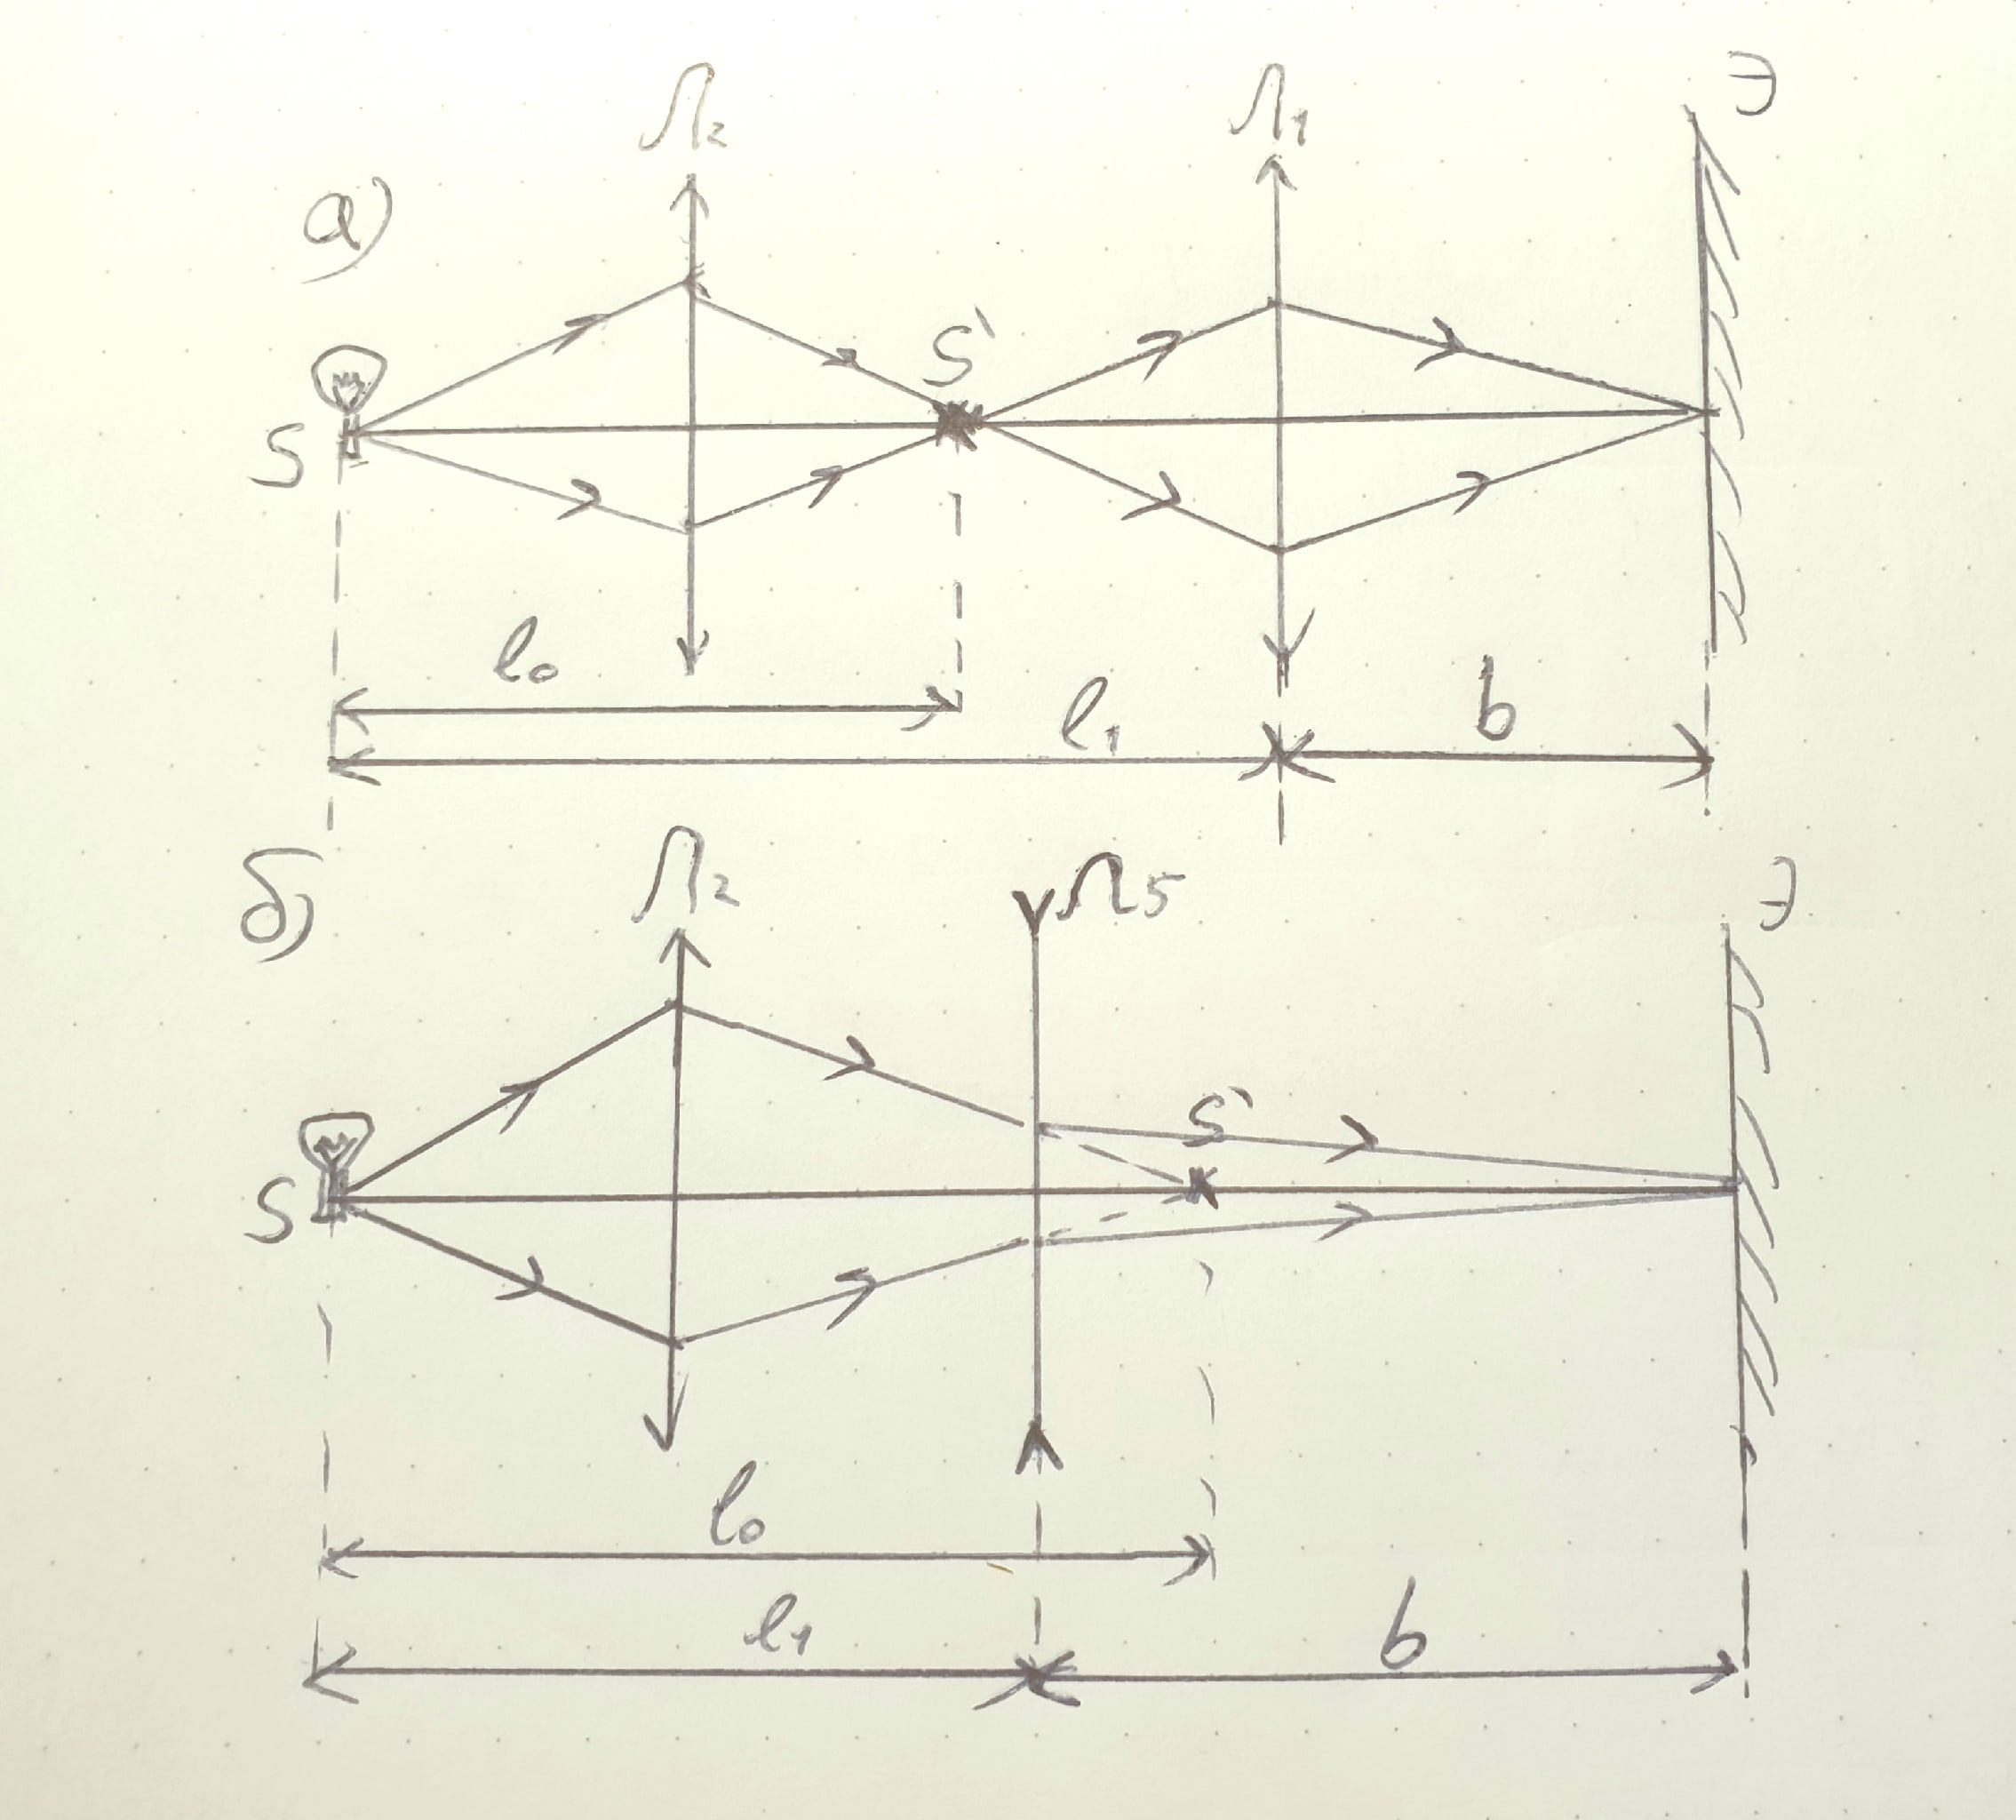
\includegraphics[width=0.8\textwidth]{3}
\end{center}
\ECaption{Схема определения фокусного расстояния а)собирающей линзы, и б)рассеивающей линзы. С помощью линзы 2 на фиксированном расстоянии $l_0$ фокусируется мнимый источник. Далее изображение фокусируют путем изменения положения экрана.}
\end{figure}

Расстояние $l_0 = 42.3$ см определяется непосредственно с помощью экрана, и после этого линза 2 не меняет положение. С помощью формулы тонкой линзы, в данных величинах получаем зависимость:
\begin{equation}
f = \frac{b(l_1-l_0)}{b+l_1-l_0}.
\end{equation}

Экспериментальная зависимость $b(l_1)$ представлены на таблице 3.

\begin{table}[h!]
\begin{center}
\begin{tabular}{|c|c|c|c|c|c|c|}
\hline
\rowcolor[HTML]{9698ED} 
Линза 1  & $l_1$, см & 61.4 & 58.5 & 57.3 & 54.5 & 53   \\ \hline
         & $b$, см   & 12.6 & 14.8 & 15.5 & 20.6 & 22.8 \\ \hline
\rowcolor[HTML]{9698ED} 
Линза 5. & $l_1$, см & 38.5 & 38.2 & 36.7 & 34.9 & 33.8 \\ \hline
         & $b$, см   & 8.3  & 8.7  & 15.8 & 43.1 & 60.5 \\ \hline
\end{tabular}
\ECaption{Зависимость $b(l_1)$.}
\end{center}
\end{table}

Фокусы можно найти по усреднению этих зависимостей из формулы 2. Получаем:

\[f_1 = 7.60 \pm 0.08 \text{ см},\]
\[f_5 = -8.5\pm 0.5 \text{ см}.\]

Стоит прокомментировать разброс значений для фокуса 5 линзы. Если посчитать отдельно $f$ по самому первому измерению для Л5, то он получался верным, а все остальные -- нет. Это наводит на мысль, что во время первого измерения изменилось положение линзы Л2, из-за чего остальные результаты недостоверны.

\subsection{Сравнение всех результатов}

Будет удобно сравнить фокусные расстояния линз, измеренные разными способами, показав их на одном графике $f(n)$ от номера линзы $n$. Эта зависимость показана на рисунке 4.


\begin{figure}[h!]
\begin{center}
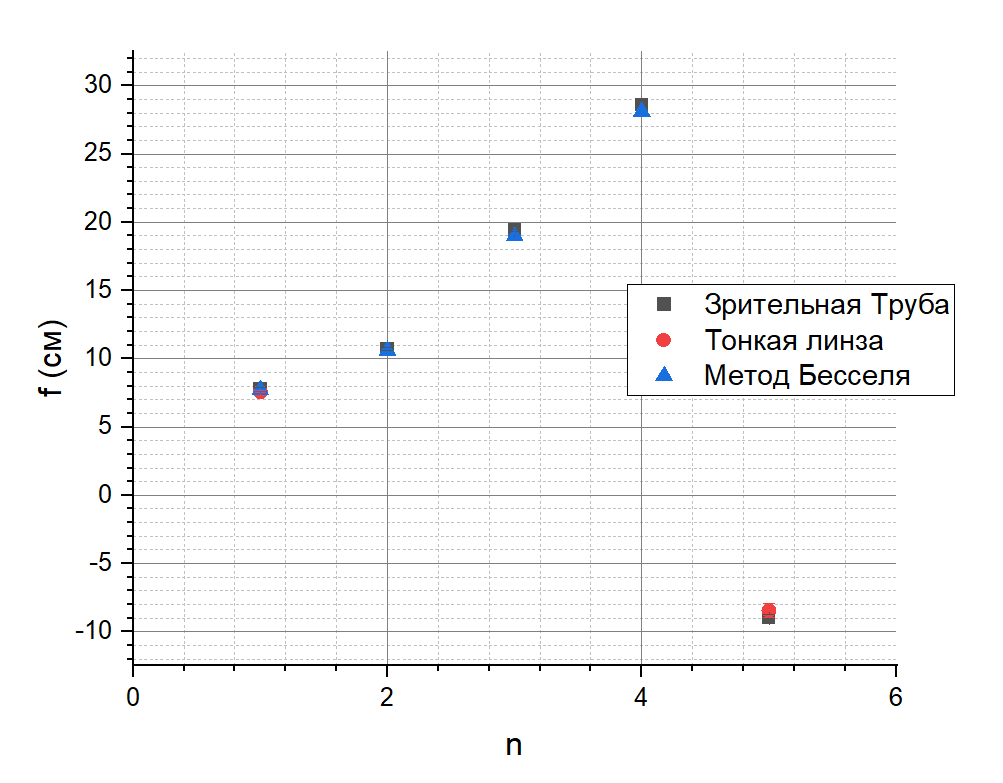
\includegraphics[width=0.8\textwidth]{gr1}
\end{center}
\ECaption{Значения фокусов для линз, измеренных разными методами. }
\end{figure}

Из этого графика видно, что сходимость результатов всех линз достаточно хорошая, что подтверждает, что приближение тонкой линзы работает в нашем эксперименте.

\section{Аберрации оптических систем}
\subsection{Сферическая аберрация}

Зависимость сферической аберрации выглядит следующим образом:
\begin{equation}
s(h) = \frac{R}{n-1}\left( 1- \frac{n^2h^2}{2R^2}\right) .
\end{equation}

Характеристической кривой сферической аберрации называют зависимость
\begin{equation}
\delta s(h) = -\frac{1}{2}\left( \frac{n}{n-1}\right)^2\left( \frac{h}{f}\right)^2 f.
\end{equation}
При $ h = r $($r$ — радиус линзы) формула (4) определяет продольную
сферическую аберрацию линзы.

Для исследования сферической аберрации использовались 3 диафрагмы диаметром $2h$, которые ставились перед линзой, и с помощью нониусной шкалы линзы, можно было измерить величину сферической аберрации $s(h)$. Данные, как водится, на таблице. 4.

\begin{table}[h!]
\begin{center}
\begin{tabular}{|c|c|}
\hline
\rowcolor[HTML]{9698ED} 
$s$, см & $h$, см \\ \hline
0.84    & 0.5     \\ \hline
\rowcolor[HTML]{9698ED} 
1       & 1       \\ \hline
1.4     & 2       \\ \hline
\end{tabular}
\ECaption{Зависимость $s$ от ширины диафрагмы (по модулю).}
\end{center}
\end{table}

Построим график $s(h^2)$, из (3) он является прямой. Тогда экстраполировав его на точку $h = r =2.5$ см -- радиус линзы, получим сферическую аберрацию. График представлен на рис.5.

\begin{figure}[h!]
\begin{center}
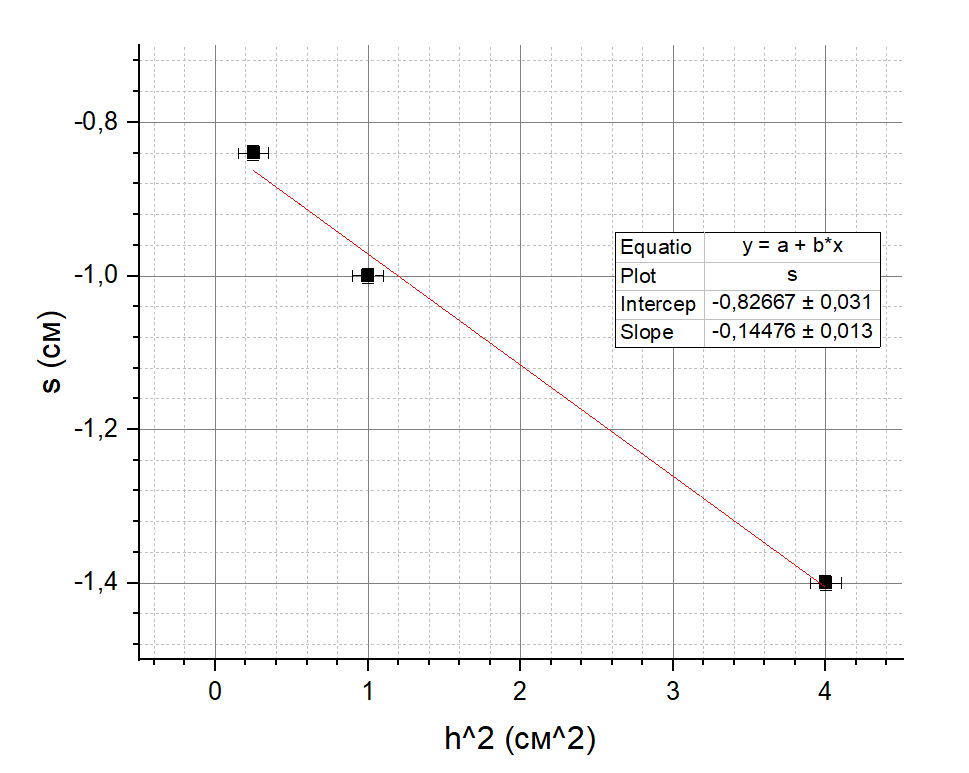
\includegraphics[width=0.8\textwidth]{gr2}
\end{center}
\ECaption{Зависимость продольной аберрации от $h^2$. Знаменитая прямая по 3 точкам. }
\end{figure}

Из графика получаем значения для коэффициентов в уравнении 
\[s(h) = bh^2 +a, \]
откуда получаем, что 
\[\delta s = br^2 = 0.91 \text{ см}. \]

Так как значение в большей степени оценочное, погрешности не существенны.

\subsection{Хроматическая аберрация}

Хроматическая аберрация (зависимость
фокусного расстояния линзы от длины волны) возникает вследствие дисперсии показателя преломления стёкол, т. е. из-за того, что показатель
преломления $n = n(\lambda).$
Хроматическую аберрацию принято
характеризовать
разностью фокусных расстояний для двух
характерных спектральных
линий водорода, располо
женных в крайних частях видимой области
спектра:
$ \lambda_F
= 486,1 $ нм (голубая линия
F водорода),
$ \lambda_C
= 656,3 $ нм
(красная линия
C водорода):
\begin{equation}
\delta f_{\text{хр}} = f_F-f_C.
\end{equation}

Для
характеристики дисперсионных свойств стёкол часто пользуются
так называемым коэффициентом дисперсии, или числом Аббе $\nu$, которое выражается через продольную хроматическую аберрацию так:
\begin{equation}
\delta f_{\text{хр}} = -\frac{1}{\nu}f_D,
\end{equation}
где $f_D$ -- фокусное расстояние для желтой линии натрия D $\lambda_D = 589.3$ нм. 
\newpage
Используя 3 светофильтра из комплекта, можно получить фокусные расстояния для каждой спектральной линии, что мы собственно сделали. Таким образом получаем:
\[\delta f_{\text{хр}} = - 1.5 \text{ мм},\]
\[\nu \approx 47.\]

\section{Вывод}

Полученные значение фокусов линз разными методами оказались одинаковы, что свидетельствует о хорошей применимости геометрической оптики в нашей работе. 

Были изучены понятия сферической и хроматической аберраций, и они были достаточно достоверно измерены для участвующей в эксперименте линзы. 

Все здорово и жизнь прекрасна.















\[x = \dfrac{\sqrt{2\hslash/m\nu}}{2}(a+a^{+}) = X_1\sqrt{2\hslash/m\nu} \]
\[p = \dfrac{\sqrt{2\hslash m\nu}}{2i}(a-a^{+}) = X_2\sqrt{2\hslash m\nu} \]
\\ \\ \\ \\ \\ \\
\[R = \frac{\lambda}{\delta\lambda}=\frac{m\beta}{2}\]



\end{document}